Motorul statistic este realizat prin integrarea unei componente care comunica cu o instanta de R 
( \url{http://www.r-project.org/} ), 
disponibila pentru prelucrari statistice.
Aceasta se bazeaza pe o interfata Java-to-R 
(implementata via JNI, Java Native Interface), 
o librarie numita rJava ( \url{http://www.rforge.net/rJava/} ).

La inceput, user-ul (clientul ExtJS) solicita serverului informatii despre o variabila sau o pereche de variabile (tab-ul "Variable Details, respectiv "Analyze"), 
iar dupa primirea raspunsului afiseaza informatiile in mod structurat (inclusiv tabele, grafice).

In cadrul proiectului Java Spring (aplicatia web cu rol de server) 
a fost dezvoltat un controller si un serviciu ce instantiaza si utilizeaza rJava 
pentru evaluarea de comenzi, functii, sau expresii in R 
(acestea fiind construite pe baza datelor importate in baza de date, ce corespund fiecarui studiu). 
Serviciul implementeaza interfata Spring SmartLifecycle pentru a putea trata pornirea si oprirea unei instante R. 
Sunt posibile operatii multiple asupra unui set de [1..N] variabile ce apartin unui studiu.
Sunt extrase si transmise ca parametri catre R metadate despre variabile, raspunsuri posibile, categorii, etichete, valori de missing, 
dar si date (valori propriu-zise ale unei variabile).

In limbajul R a fost dezvoltat un set de functii parametrizate 
(ce sunt incarcate si apelate la runtime din layer-ul de servicii al aplicatiei web server).
Unele dintre aceste functii construiesc raspunsul (fie structurat, fie nestructurat - ca sir de caractere) 
pe care aplicatia il trimite mai departe catre clientul ExtJS (in format JSON).

Mai jos sunt prezentate imagini ale de acces la date, in care se pot vedea (in partea dreapta-jos) 
rezultatele obtinute de la motorul statistic pentru analiza unei variabile, respectiv a doua variabile.

\medskip
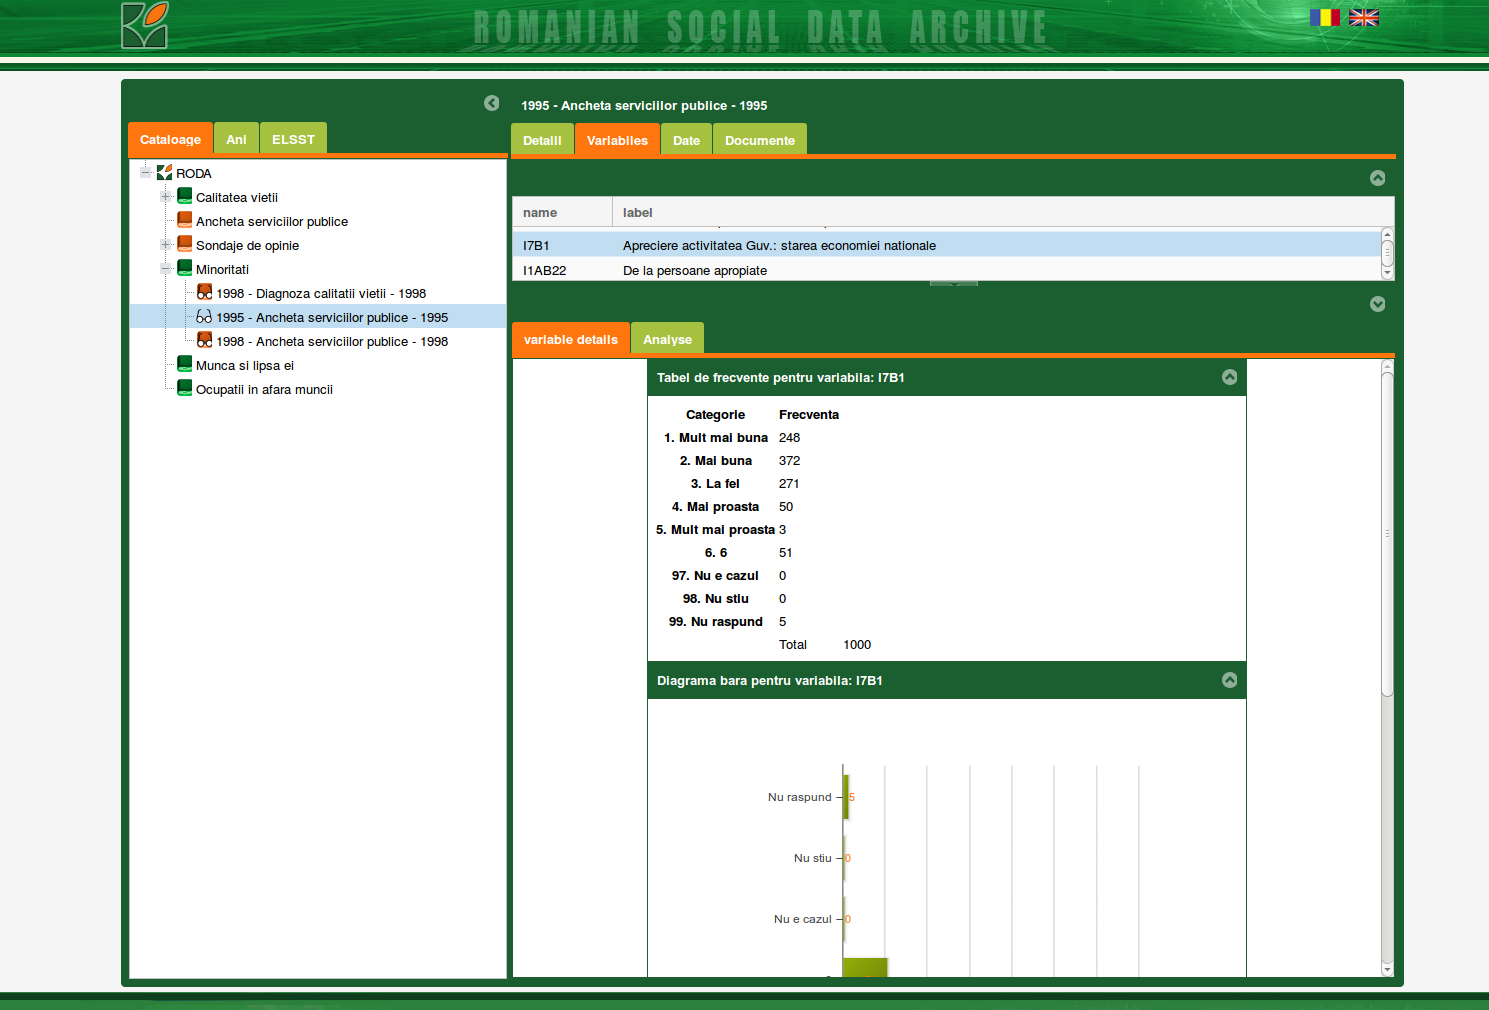
\includegraphics[width=\textwidth]{img/Screenshot-statistics}

\medskip
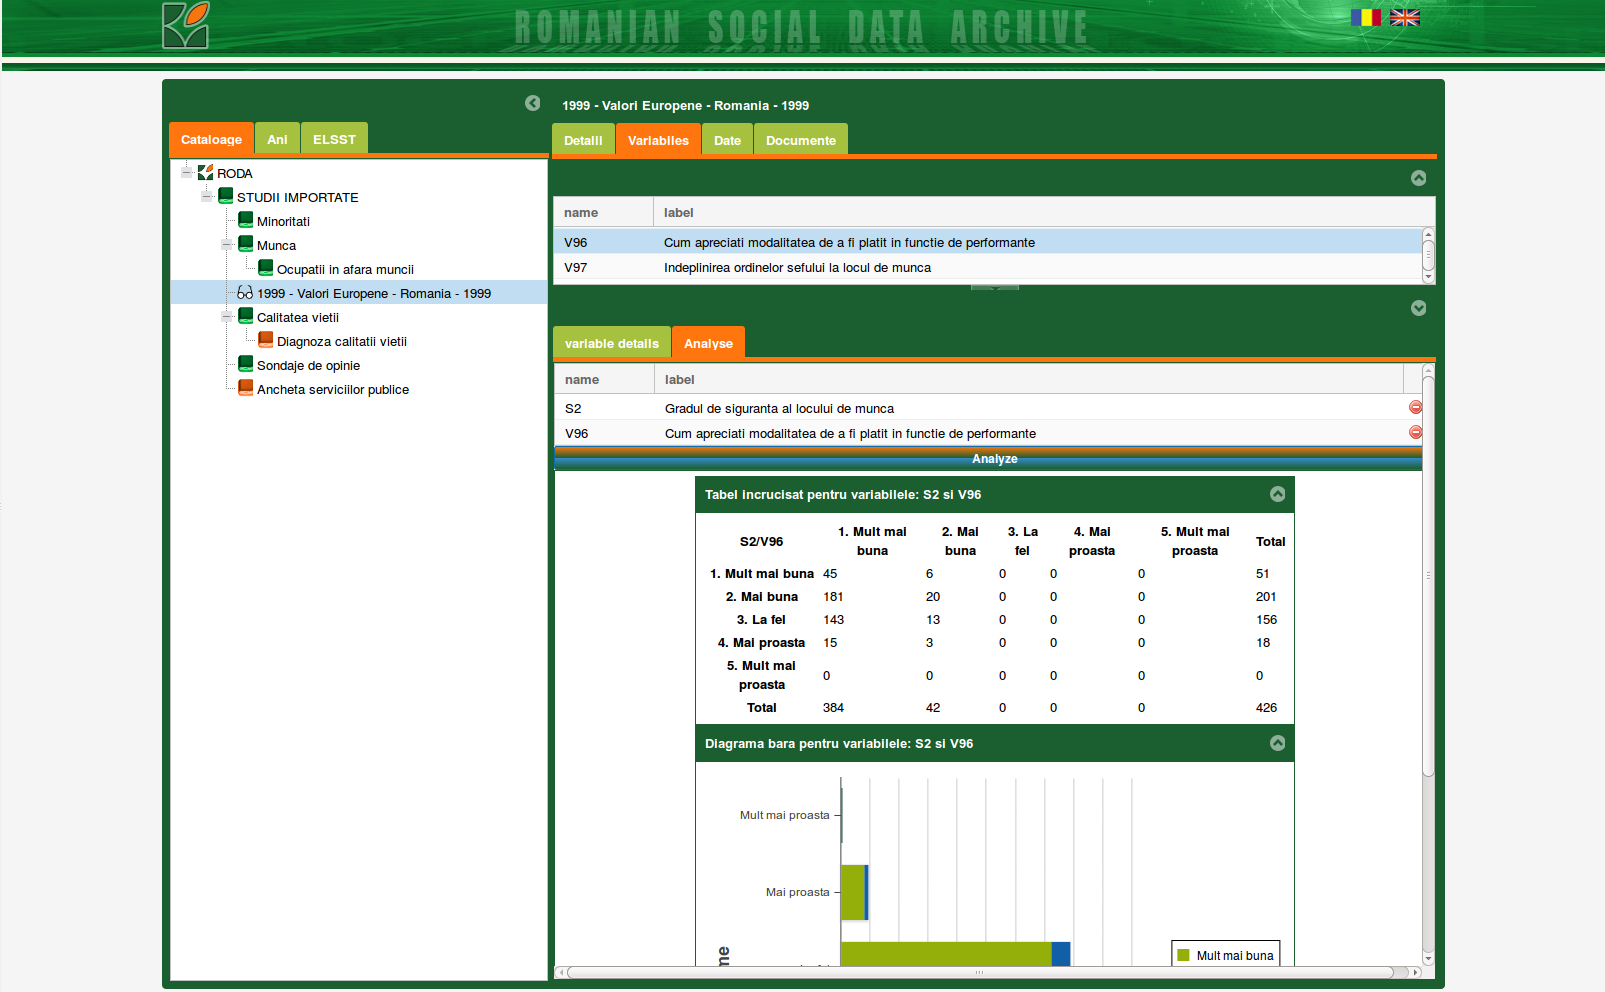
\includegraphics[width=\textwidth]{img/Screenshot-statistics-analyze}
